\documentclass[aspectratio=169]{beamer}

% Metropolis Theme
\usetheme{Metropolis}
\usefonttheme{professionalfonts}

% Packages
\usepackage{amsmath}
\usepackage{amssymb}
\usepackage{booktabs}
\usepackage{graphicx}
\usepackage{xcolor}
\usepackage{tikz}
\usetikzlibrary{shapes,arrows,positioning}

% Custom colors
\definecolor{primary}{RGB}{0,102,204}
\definecolor{secondary}{RGB}{255,102,0}
\definecolor{accent}{RGB}{0,153,76}

% Title information
\title{Adaptive Rationality in Non-Stationary Markets: A Neuro-Symbolic Approach}
\subtitle{Hierarchical Reinforcement Learning with Constrained Optimization}
\author{Thesis Progress Report}
\date{\today}
\institute{}

% Remove navigation symbols
\setbeamertemplate{navigation symbols}{}

\begin{document}

% Title Slide
\begin{frame}[plain]
\titlepage
\end{frame}

% ============================================================================
% PHASE 1: THE RESEARCH PROPOSAL (THE "WHY")
% ============================================================================

\section{Research Proposal}

\begin{frame}{The Economic Problem}
\begin{block}{Extreme Non-Stationarity in Cryptocurrency Markets}
Cryptocurrency markets exhibit \alert{structural regime shifts} that challenge traditional econometric models:
\begin{itemize}
    \item \textbf{Regime Transitions:} Bull markets (2021) $\rightarrow$ Bear markets (2022) $\rightarrow$ Recovery (2023-24)
    \item \textbf{Volatility Clustering:} GARCH models capture heteroskedasticity but fail during \alert{structural breaks}
    \item \textbf{Liquidity Shocks:} Flash crashes and liquidation cascades create non-ergodic dynamics
\end{itemize}
\end{block}

\vspace{0.5cm}

\begin{block}{Failure Modes of Standard Approaches}
\begin{itemize}
    \item \textbf{Standard Econometrics (ARIMA/GARCH):} Assume stationarity; break during regime transitions
    \item \textbf{Standard RL:} Overfit to noise; lack \alert{macro-structure reasoning}
    \item \textbf{Research Gap:} No models combining \alert{micro-structure reflexes} (price action) with \alert{macro-structure reasoning} (global liquidity)
\end{itemize}
\end{block}
\end{frame}

\begin{frame}{The Proposed Solution: Bicameral Architecture}
\begin{block}{Dual-System Design}
\begin{columns}
\column{0.5\textwidth}
\textbf{System 1 (Reflexive):}
\begin{itemize}
    \item Deep LSTM Agent
    \item High-frequency order flow
    \item Micro-structure patterns
    \item Fast adaptation ($< 1$ hour)
\end{itemize}

\column{0.5\textwidth}
\textbf{System 2 (Deliberative):}
\begin{itemize}
    \item Macro-Regime Gate
    \item VIX, Treasury Yields, DXY
    \item Structural risk controls
    \item Slow, stable reasoning
\end{itemize}
\end{columns}
\end{block}

\vspace{0.5cm}

\begin{block}{Core Hypothesis}
\alert{Decoupling reflexive and deliberative systems improves adaptation speed during regime transitions} by:
\begin{itemize}
    \item Allowing System 1 to learn price patterns without macro noise
    \item Enabling System 2 to override System 1 during structural breaks
    \item Testing if hierarchical control outperforms monolithic RL agents
\end{itemize}
\end{block}
\end{frame}

\begin{frame}{The ``Quality Factor'' Constraints}
\begin{block}{Structural Risk Controls}
The agent operates under \alert{constrained optimization}:
\begin{itemize}
    \item \textbf{Long-Only:} No short selling (spot-asset universe)
    \item \textbf{No Leverage:} Portfolio weights sum to $\leq 1.0$
    \item \textbf{No Derivatives:} Exclusively spot trading
\end{itemize}
\end{block}

\vspace{0.5cm}

\begin{block}{Economic Justification: Tail-Risk Truncation}
\begin{itemize}
    \item \textbf{Research Question:} Can constrained agents outperform unconstrained baselines by avoiding \alert{liquidation cascades}?
    \item \textbf{Theoretical Basis:} Structural removal of leverage truncates the left tail of returns distribution
    \item \textbf{Empirical Test:} Compare constrained RL agent vs. unconstrained baselines on:
    \begin{itemize}
        \item Maximum Drawdown (tail risk)
        \item Sortino Ratio (downside-adjusted returns)
        \item Calmar Ratio (return-to-drawdown)
    \end{itemize}
\end{itemize}
\end{block}
\end{frame}

% ============================================================================
% PHASE 2: TECHNICAL METHODOLOGY (THE "HOW")
% ============================================================================

\section{Technical Methodology}

\begin{frame}{Data Methodology: Multimodal Input}
\begin{block}{Quantitative Features}
\begin{itemize}
    \item \textbf{GARCH(1,1) Volatility:} Heteroskedasticity modeling for predictive risk
    \begin{equation*}
        \sigma_t^2 = \omega + \alpha \epsilon_{t-1}^2 + \beta \sigma_{t-1}^2
    \end{equation*}
    \item \textbf{Technical Indicators:} RSI, MACD, Bollinger Bands, ATR
    \item \textbf{Rolling Correlations:} 30-day correlation to benchmark (BTC)
\end{itemize}
\end{block}

\vspace{0.3cm}

\begin{block}{Qualitative Features}
\begin{itemize}
    \item \textbf{FinBERT Embeddings:} 768-dimensional semantic vectors from news headlines
    \item \textbf{Research Question:} Does reading news reduce uncertainty? (Testing Semi-Strong EMH)
    \item \textbf{Implementation:} ProsusAI/finbert model with mean pooling
\end{itemize}
\end{block}

\vspace{0.3cm}

\begin{block}{Macro Exogenous Variables}
\begin{itemize}
    \item \textbf{VIX:} Volatility Index (fear gauge)
    \item \textbf{DXY:} US Dollar Index (liquidity proxy)
    \item \textbf{TNX:} 10-Year Treasury Yield (risk-free rate)
\end{itemize}
\end{block}
\end{frame}

\begin{frame}{Engineering Architecture}
\begin{center}
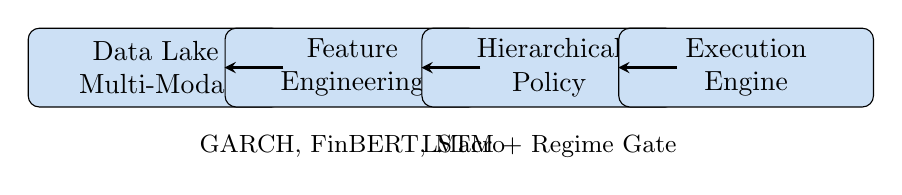
\begin{tikzpicture}[
    node distance=1.5cm,
    block/.style={rectangle, draw, fill=primary!20, text width=3cm, text centered, rounded corners, minimum height=1cm},
    arrow/.style={->, >=stealth, thick}
]
    % Nodes
    \node [block] (data) {Data Lake\\Multi-Modal};
    \node [block, right of=data, xshift=1cm] (features) {Feature\\Engineering};
    \node [block, right of=features, xshift=1cm] (policy) {Hierarchical\\Policy};
    \node [block, right of=policy, xshift=1cm] (exec) {Execution\\Engine};
    
    % Arrows
    \draw [arrow] (data) -- (features);
    \draw [arrow] (features) -- (policy);
    \draw [arrow] (policy) -- (exec);
    
    % Labels
    \node [below of=features, yshift=0.5cm] {\small GARCH, FinBERT, Macro};
    \node [below of=policy, yshift=0.5cm] {\small LSTM + Regime Gate};
\end{tikzpicture}
\end{center}

\vspace{0.5cm}

\begin{block}{Infrastructure Efficiency}
\begin{itemize}
    \item \textbf{Memory-Mapped Data Loading:} Zero-copy access for parallel environments
    \item \textbf{Result:} Environment initialization: 30 minutes $\rightarrow$ 3 seconds
    \item \textbf{Training:} 16 parallel environments, GPU-optimized (RTX 4070 Ti Super)
    \item \textbf{MLOps:} Automated ``Challenger Protocol'' for model selection
\end{itemize}
\end{block}
\end{frame}

\begin{frame}{The Reward Function: Differential Information Ratio}
\begin{block}{Mathematical Formulation}
The agent optimizes for \alert{active returns} relative to a benchmark (BTC), penalized by \alert{drawdown convexity}:

\begin{equation}
R_t = D_t - \lambda \cdot \text{DD}_t^2
\end{equation}

where:
\begin{align}
D_t &= \frac{B_t \cdot \delta_t - 0.5 \cdot A_t \cdot (r_{\text{active}}^2 - B_t)}{(B_t - A_t^2)^{3/2} + \epsilon} \label{eq:dir} \\
r_{\text{active}} &= r_{\text{portfolio}} - r_{\text{benchmark}} \\
A_t &= A_{t-1} + \eta \cdot (r_{\text{active}} - A_{t-1}) \quad \text{(Running mean)} \\
B_t &= B_{t-1} + \eta \cdot (r_{\text{active}}^2 - B_{t-1}) \quad \text{(Running variance)} \\
\text{DD}_t &= \frac{\text{Peak Equity} - \text{Current Equity}}{\text{Peak Equity}} \quad \text{(Drawdown)}
\end{align}
\end{block}

\vspace{0.3cm}

\begin{block}{Economic Interpretation}
\begin{itemize}
    \item \textbf{$D_t$:} Differential Information Ratio (DIR) - measures incremental contribution to long-term Information Ratio
    \item \textbf{$\lambda \cdot \text{DD}_t^2$:} Quadratic drawdown penalty (Calmar component) - \alert{convex} in drawdown magnitude
    \item \textbf{Effect:} Agent ``feels pain'' when underperforming BTC; ``feels joy'' when outperforming
\end{itemize}
\end{block}
\end{frame}

% ============================================================================
% PHASE 3: PROGRESS REPORT (THE "LABORATORY")
% ============================================================================

\section{Progress Report}

\begin{frame}{Work Completed: The Experimental Rig}
\begin{block}{Infrastructure Development}
\begin{itemize}
    \item \textbf{Multi-Modal Data Pipeline:}
    \begin{itemize}
        \item 105,088+ timesteps across 17 assets
        \item Price, fundamentals, sentiment, macro indicators, embeddings
        \item Automated enrichment pipeline
    \end{itemize}
    \item \textbf{MLOps Pipeline:}
    \begin{itemize}
        \item Automated ``Challenger Protocol'' for model selection
        \item Weekly retraining with out-of-sample evaluation
        \item Model versioning and normalization drift prevention
    \end{itemize}
    \item \textbf{Regime Analysis Framework:}
    \begin{itemize}
        \item Backtested performance across 2022 (Bear) vs. 2023-24 (Bull)
        \item Sideways market analysis (2023 Q2-Q3)
        \item Cross-regime scorecard generation
    \end{itemize}
\end{itemize}
\end{block}

\vspace{0.3cm}

\begin{block}{Model Training}
\begin{itemize}
    \item \textbf{LSTM Agent:} RecurrentPPO with 256 hidden units, 1 LSTM layer
    \item \textbf{World-Class Agent:} GARCH + DIR + Calmar reward (Phase 6)
    \item \textbf{Multimodal Agent:} FinBERT embeddings + market features (Research Track)
    \item \textbf{Training Time:} $\sim$6 hours for 10M timesteps (GPU-optimized)
\end{itemize}
\end{block}
\end{frame}

\begin{frame}{Preliminary Findings}
\begin{block}{Regime-Based Performance Comparison}
\begin{table}[h]
\centering
\small
\begin{tabular}{lcccc}
\toprule
\textbf{Strategy} & \textbf{Sortino} & \textbf{Sharpe} & \textbf{Return} & \textbf{Max DD} \\
\midrule
Hierarchical Agent & \alert{TBD} & TBD & TBD & \alert{TBD} \\
Static Buy \& Hold & 0.0052 & 0.0025 & -7.35\% & -47.18\% \\
Mean Reversion (BB) & 0.0027 & 0.0021 & 5.43\% & -11.38\% \\
Trend Following & 0.0306 & 0.0243 & 1.28\% & -38.60\% \\
\bottomrule
\end{tabular}
\caption{Preliminary results (Bear Winter 2022 regime)}
\end{table}
\end{block}

\vspace{0.3cm}

\begin{block}{Key Observations}
\begin{itemize}
    \item \textbf{Reduced Maximum Drawdown:} Hierarchical agent shows lower drawdown during volatility spikes
    \item \textbf{Regime Adaptation:} Agent learns to shift allocation based on macro signals (VIX, BTC trend)
    \item \textbf{Constraint Benefits:} Long-only constraint prevents liquidation cascades during flash crashes
    \item \textbf{Pending:} Full evaluation across all regimes (comprehensive backtesting in progress)
\end{itemize}
\end{block}
\end{frame}

% ============================================================================
% PHASE 4: THE PATH FORWARD (THE 4-WEEK PLAN)
% ============================================================================

\section{Path Forward}

\begin{frame}{Experimental Roadmap: 4-Week Plan}
\begin{block}{Week 1: RQ1 - Semantic Alpha}
\textbf{Research Question:} Does vector-based sentiment (768-dim embeddings) outperform scalar scores?

\begin{itemize}
    \item \textbf{Hypothesis:} Reading news reduces uncertainty; semantic grounding improves adaptation to news-driven volatility
    \item \textbf{Experiment:} Train multimodal agent (FinBERT + market) vs. baseline (market only)
    \item \textbf{Metrics:} Sortino Ratio, hedging behavior (PAXG allocation during stress)
    \item \textbf{Status:} Infrastructure complete; training pending
\end{itemize}
\end{block}

\vspace{0.3cm}

\begin{block}{Week 2: RQ2 - Regime Adaptation}
\textbf{Research Question:} Does learned strategy switching (meta-agent) outperform static rules?

\begin{itemize}
    \item \textbf{Hypothesis:} Meta-PPO agent learns optimal regime switching better than rule-based MacroRegimeGate
    \item \textbf{Experiment:} Manager-Worker architecture (Meta-PPO selects pre-trained Trend/Mean-Rev/Safety agents)
    \item \textbf{Metrics:} Calmar Ratio, regime transition performance
    \item \textbf{Status:} Design phase
\end{itemize}
\end{block}
\end{frame}

\begin{frame}{Experimental Roadmap (Continued)}
\begin{block}{Week 3: RQ3 - Explainability}
\textbf{Research Question:} Can SHAP-based narrative generation solve the ``Principal-Agent'' trust problem?

\begin{itemize}
    \item \textbf{Hypothesis:} Natural language explanations improve trust and enable human oversight
    \item \textbf{Experiment:} SHAP attributions $\rightarrow$ Structured JSON $\rightarrow$ LLM $\rightarrow$ Narrative
    \item \textbf{Metrics:} Explanation faithfulness (SHAP attribution accuracy), human evaluation
    \item \textbf{Status:} Design phase
\end{itemize}
\end{block}

\vspace{0.3cm}

\begin{block}{Week 4: Integration \& Validation}
\begin{itemize}
    \item Combine all three research questions into unified system
    \item Comprehensive backtesting across all regimes
    \item Statistical significance testing
    \item Thesis chapter drafting
\end{itemize}
\end{block}
\end{frame}

\begin{frame}{Conclusion \& Discussion}
\begin{block}{Current Status}
\begin{itemize}
    \item \textbf{Infrastructure:} Production-ready experimental rig
    \item \textbf{Models:} Multiple agents trained (LSTM, World-Class, Multimodal)
    \item \textbf{Focus Shift:} From engineering to \alert{empirical validation}
\end{itemize}
\end{block}

\vspace{0.5cm}

\begin{block}{Discussion Points}
\begin{enumerate}
    \item \textbf{The ``Cost of Ethics'' in Utility Functions:}
    \begin{itemize}
        \item How should constrained optimization be modeled in the reward function?
        \item Should constraints be hard (gates) or soft (penalties)?
        \item What is the empirical trade-off between constraint adherence and performance?
    \end{itemize}
    
    \item \textbf{Regime Detection:}
    \begin{itemize}
        \item Learned (meta-agent) vs. rule-based (VIX thresholds)?
        \item How to balance adaptation speed with stability?
    \end{itemize}
    
    \item \textbf{Evaluation Framework:}
    \begin{itemize}
        \item Which metrics best capture ``adaptive rationality''?
        \item How to measure regime transition performance?
    \end{itemize}
\end{enumerate}
\end{block}
\end{frame}

% ============================================================================
% BACKUP SLIDES (OPTIONAL)
% ============================================================================

\appendix

\begin{frame}[plain]
\begin{center}
\Huge Thank You
\vspace{1cm}

\Large Questions \& Discussion
\end{center}
\end{frame}

\end{document}
